\section{Overflow Handling}

In normal process, output \(Z\) is a 24-bit unsigned number from the equation since \(A\) and \(B\) are 8-bit numbers.
Here are two methods to convert 24-bit unsigned number into 16-bit signed number.

\subsection{Method 1: Negation Output}

\subsubsection{Overflow Detection}

To detect whether a 24-bit unsigned number is overflow for a 16-bit signed slot,
just simply using a 9-bit or gate for the higher 9-bit of the 24-bit unsigned number.

The RTL description is shown in \figref{fig:zero_det_rtl} and the simulation result of block is shown in \figref{fig:zero_det_sim}.

\begin{figure}[!ht]
	\centering
	\caption{Synthesized RTL Diagram of the Zero Detector}
	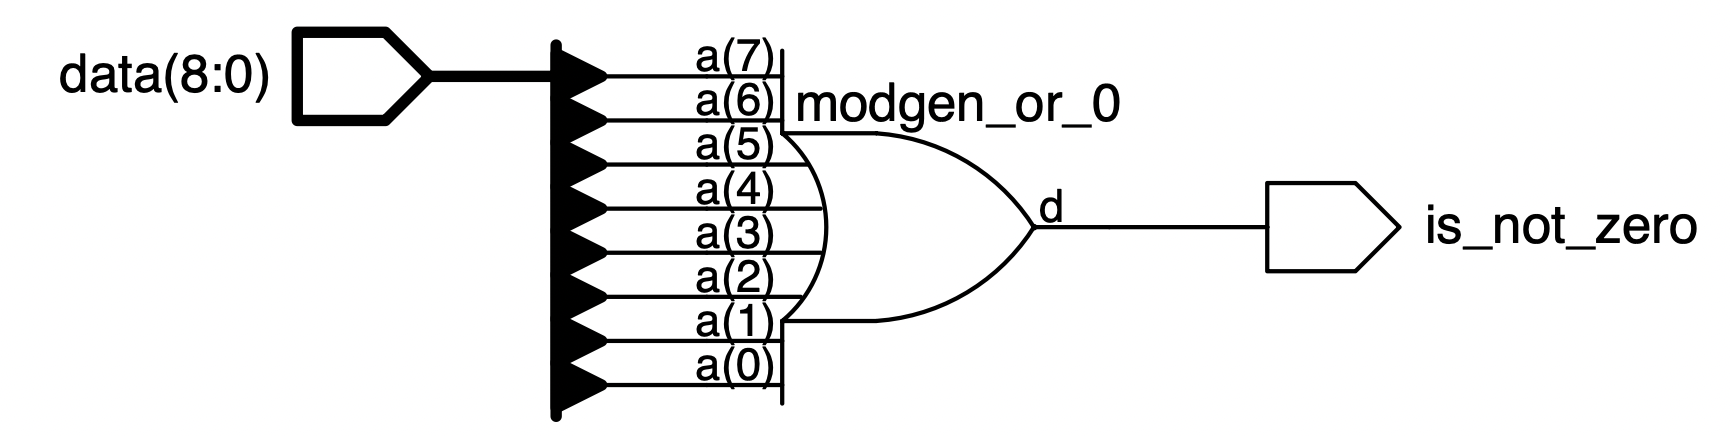
\includegraphics[width=0.6\textwidth]{../img/zero_det_rtl.png}
	\label{fig:zero_det_rtl}
\end{figure}

\begin{figure}[!ht]
	\centering
	\caption{Simulation Wave Diagram of the Zero Detector}
	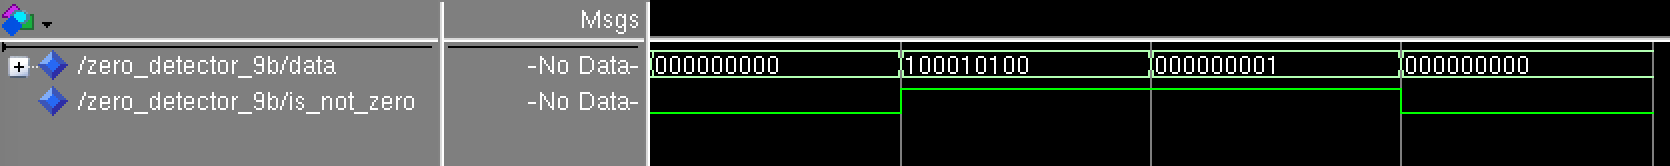
\includegraphics[width=0.9\textwidth]{../img/zero_det_sim.png}
	\label{fig:zero_det_sim}
\end{figure}

\subsubsection{Handler Implementation}

Once the 24-bit result is detected as an overflowing number,
the circuit will just output a negative number to indicate the overflow happens.
The RTL description of the implementation is shown in \figref{fig:neg_rtl} and the simulation result of block is shown in \figref{fig:neg_sim}.

\begin{figure}[!ht]
	\centering
	\caption{Synthesized RTL Diagram of the Overflow Handler of Method 1}
	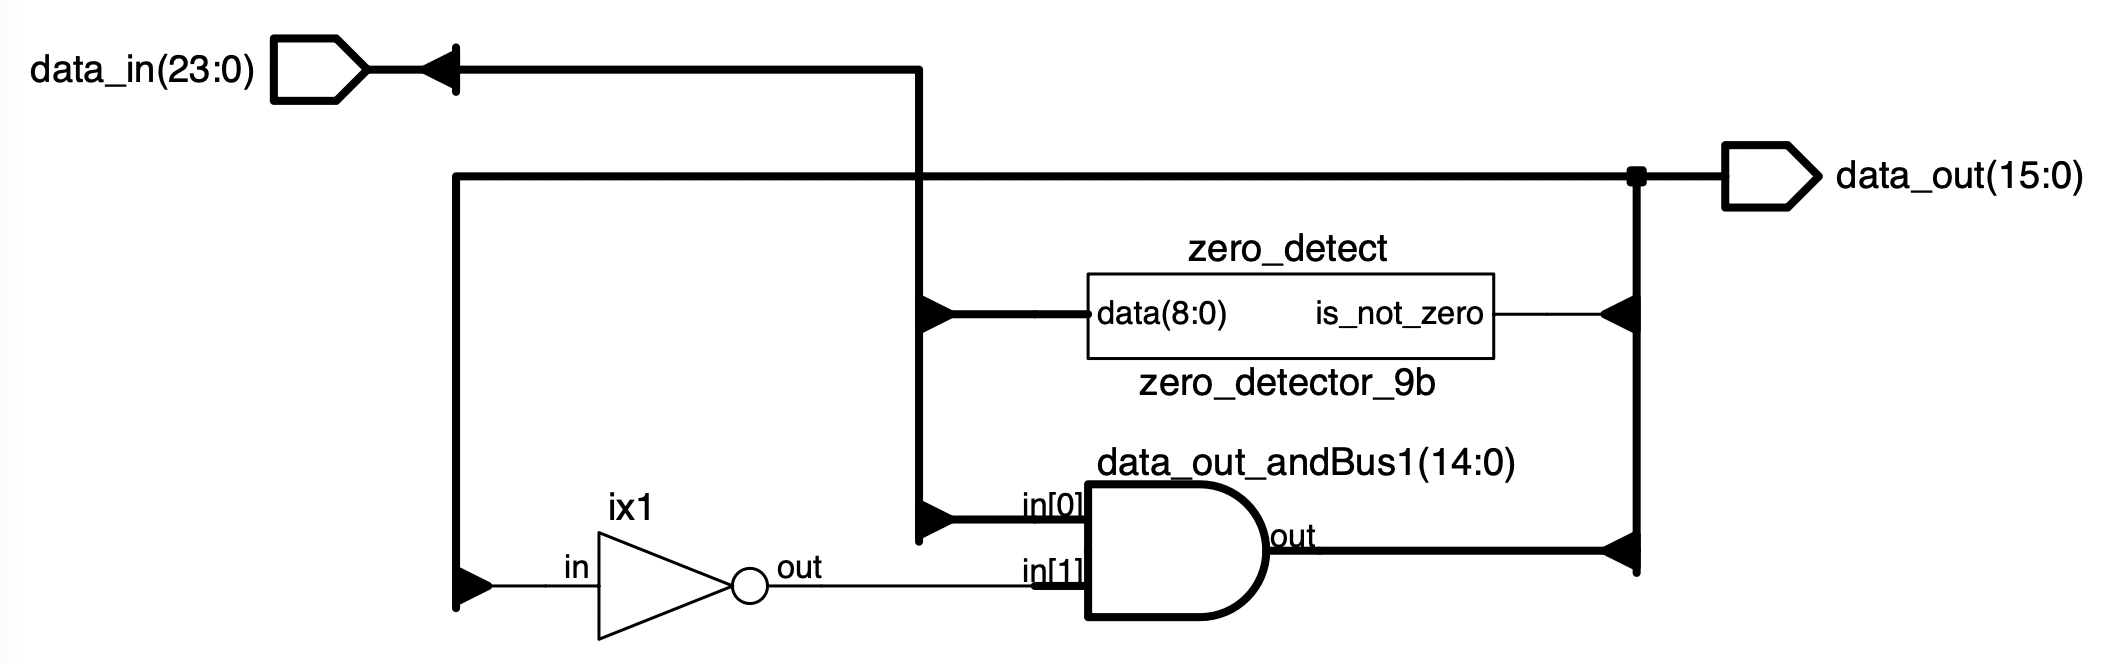
\includegraphics[width=0.7\textwidth]{../img/neg_rtl.png}
	\label{fig:neg_rtl}
\end{figure}

\begin{figure}[!ht]
	\centering
	\caption{Simulation Wave Diagram of the Overflow Handler of Method 1}
	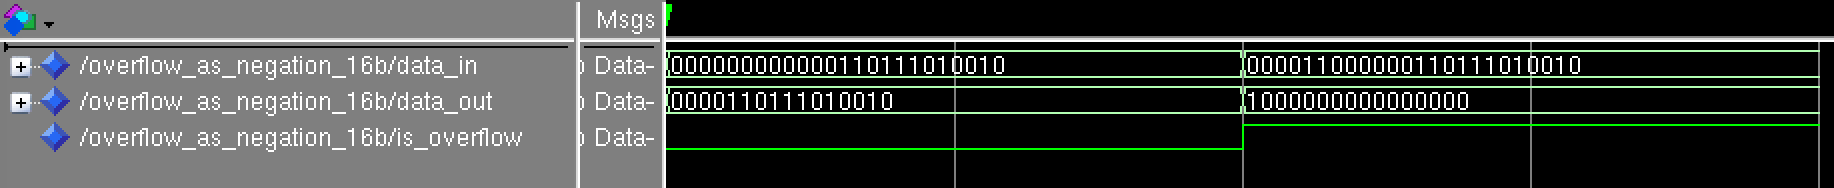
\includegraphics[width=0.9\textwidth]{../img/neg_sim.png}
	\label{fig:neg_sim}
\end{figure}

\subsection{Method 2: Display Z Separately with Two Clock Cycles}

In this method, the circuit will output the 24-bit number into two parts.
The higher part of the 24-bit result which is a 9-bit number
will be stored in a register with concatenating a \textquote{1000000} to its front;
The rest of the 15-bit will be stored in another register with concatenating a \textquote{0} to its front.
Then the circuit will output those two parts to \(Z\) alternately by the clock cycles.

The drawback of this method is obvious: \textbf{the result will need two clock cycles to be fully obtained}.
Hence the input of the ALU circuit should have a clock of the time interval between every set of \(A\) and \(B\) input
to avoid output overlaps.
This method acts like a 2 states FSM which RTL description is shown in \figref{fig:sep_display_rtl}.
The simulation result of block is shown in \figref{fig:sep_display_sim}.

\begin{figure}[!ht]
	\centering
	\caption{Synthesized RTL Diagram of the Overflow Handler of Method 2}
	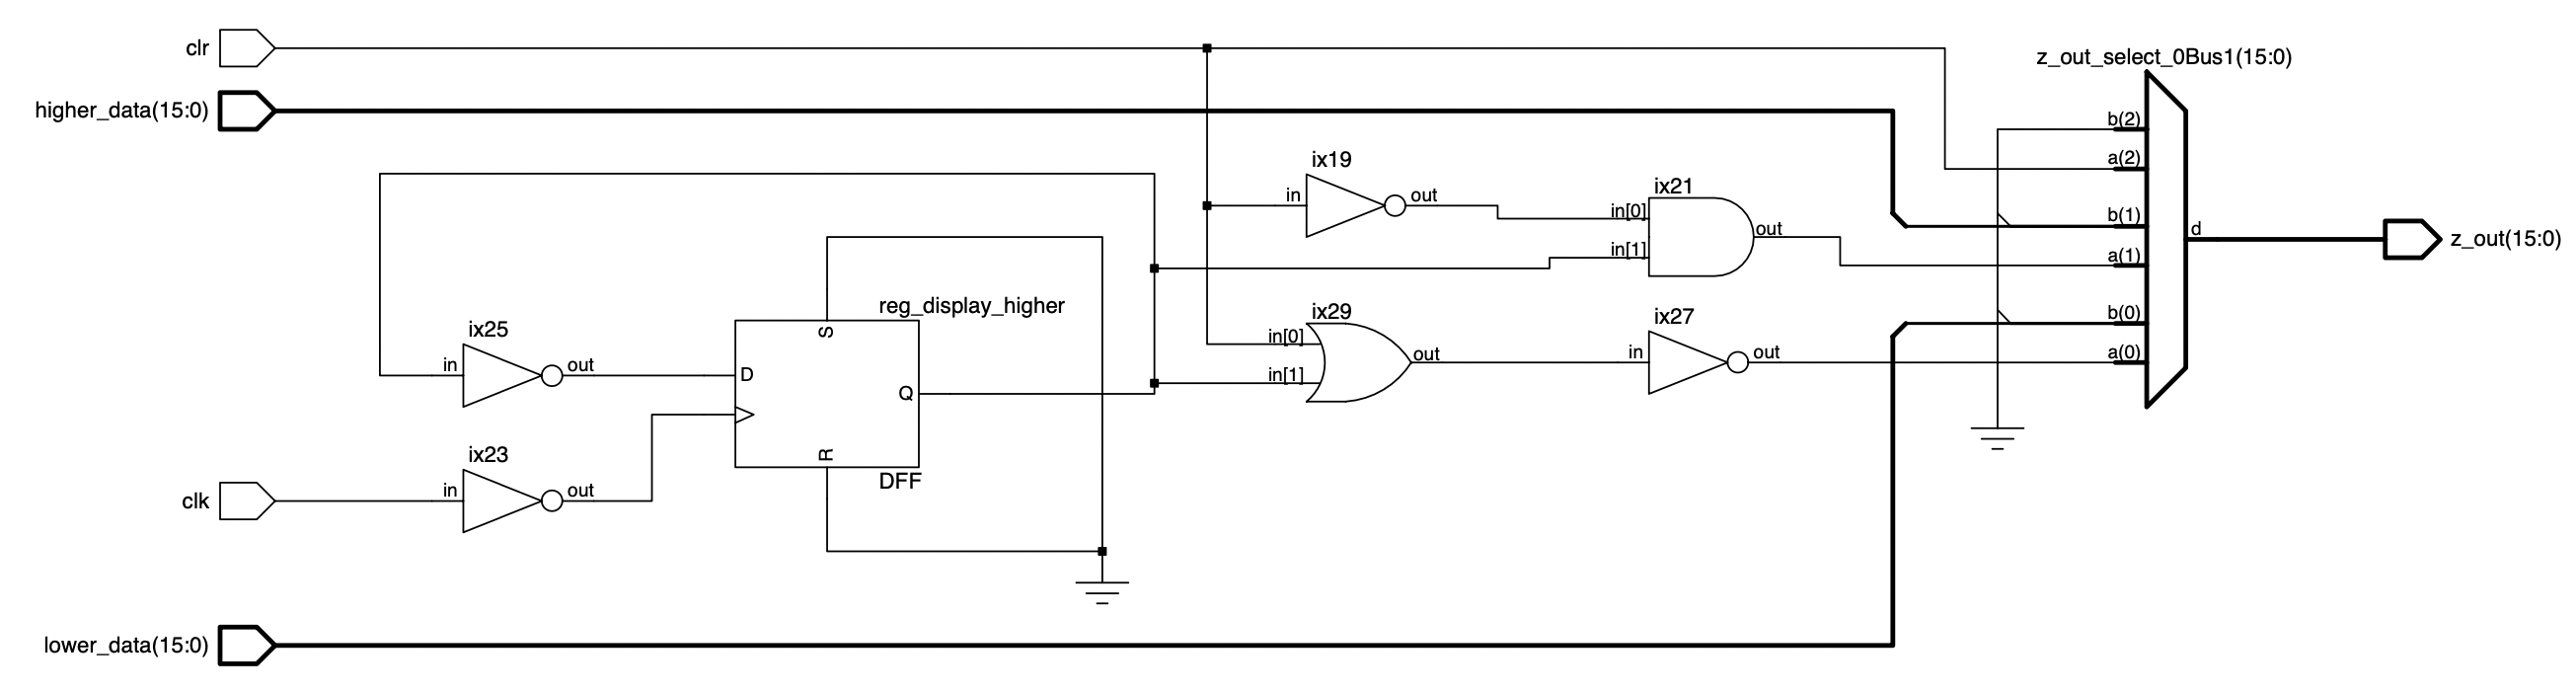
\includegraphics[width=\textwidth]{../img/sep_display_rtl.png}
	\label{fig:sep_display_rtl}
\end{figure}

\begin{figure}[!ht]
	\centering
	\caption{Simulation Wave Diagram of the Overflow Handler of Method 2}
	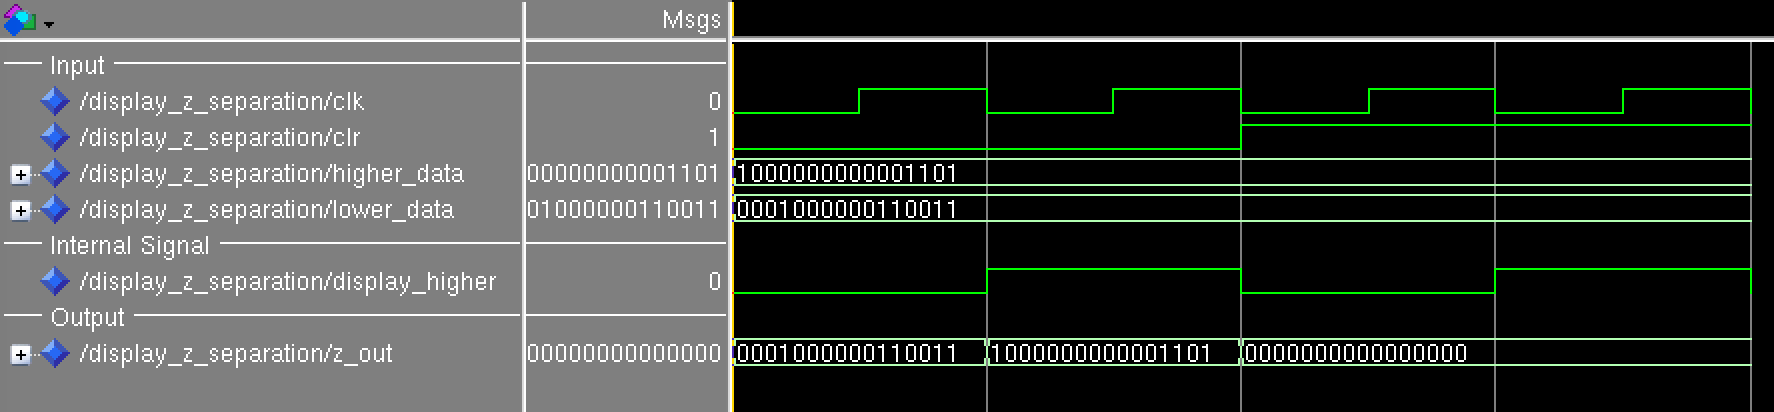
\includegraphics[width=0.8\textwidth]{../img/sep_display_sim.png}
	\label{fig:sep_display_sim}
\end{figure}